\section{Modernien anturiverkkojen tiedonsiirto-ongelmat}
\TODO{Selitä tarkasti mitä ongelmaa artikkelit ryhtyvät ratkaisemaan}

Anturiverkkojen toimintaolosuhteista johtuen verkon yhteydet ovat muuttuvia ja
ennalta-arvaamattomia. Usein verkon yksittäisillä antureilla ei ole tietoa
verkon koostumuksesta sen välittömien naapureiden lisäksi. Siksi
reititysprotokollien täytyy pystyä sopeutumaan muuttuviin tilanteisiin
mahdollisimman vähällä informaatiolla itse verkosta.

Ensimmäinen artikkeli keskittyy anturiverkkojen keräämän datan tehokkaaseen
yhdistämiseen, eli datafuusioon. Toinen taas pyrkii kehittämään
reititysprotokollan joka on robusti ja pystyy mukautumaan antureiden
tuhoutumisesta johtuviin muutoksiin.

\subsection{Datafuusio}
Artikkelissa~\cite{Yu2006} keskeistä on anturien keräämän datan fuusio.
Datafuusio tarkoittaa toisiinsa liittyvän datan liittämistä yhteen. Artikkeli
käyttää esimerkkinä UAV:sta koostuvaa anturiverkkoa, joissa jokaisella
yksittäisellä UAV:lla on matala varmuus kokonaistilanteesta. Datafuusio on
tärkeää jotta verkolla on vahva käsitys tilanteesta jonka avulla se voi
suunnitella toimintaansa.

Datafuusio toimii niin että toisiinsa liittyvä data koitetaan kerätä yhteen.
Verkon nodet lähettävät dataa eteenpäin kunnes jollakin nodella on tarpeeksi
paljon dataa, jolloin se lopettaa datan eteenpäinlähetyksen ja rupeaa
prosessoimaan dataa ja tekemään sen avulla päätöksiä.

\subsection{Luotettava tiedonsiirto anturiverkoissa}
Anturiverkon osien, eli ``nodejen'' kuolemat ovat ongelma jonka verkon täytyy
pystyä kestämään ja käsittelemään. Kuolema tarkoittaa tässä kontekstissa mitä
tahansa tilannetta jossa node on toimintakyvytön tai sen toimintakyky on niin
huono että siitä ei ole hyötyä verkossa. Artikkelissa~\cite{Arya2015} esitelty
algoritmi pyrkii etsimään nodejen kuolemista syntyviä ``reikiä'' ja reitittämään
data optimaalisesti ne huomioon ottaen.

\subsection{Muita anturiverkkojen reititysalgoritmeja}
\TODO{Kerro joistain muista reititysprotokollista, ja siitä miksi ne eivät
sovellu kuitenkaan tässä esitettyihin ongelmiin}

\section{Vahvistumisoppiminen anturiverkojen tiedonsiirrossa}
\TODO{Selitä tarkasti miten em ongelma ratkaistaan vahvistusoppimista käyttäen}

Kummatkin artikkelit siis ryhtyvät ratkaisemaan anturiverkkojen tiedonsiirron
reitityksen optimointia. Molemmat myös pyrkivät löytämään nopeita ja
luotettavia yhteyksiä nodejen väleille. Ensimmäinen kuitenkin pyrkii pääasiassa
etsimään verkon reikiä ja toinen pyrkii optimoimaan datafuusiota.

\TODO{Mitä vahvistusoppiminen on?}

\subsection{Datan tehokas yhdistäminen vahvistusoppimisen avulla}

Yksinkertainen algoritmi datan yhdistämiseen anturiverkossa on niin sanottu
``path reinforcement'' algoritmi, jonka toimintaa havainnollistaa
kuva~\ref{fig:yu2006}. Kun algoritmi ensimmäisen kerran saa dataa tietystä
tapahtumasta, se lähettää sen satunnaiselle naapurille eteenpäin. Kun se saa
samasta tapahtumasta lisää dataa, se lähettää sen eteenpäin sille naapurille
jolle se viimeksi lähetti dataa kyseisestä tapahtumasta.  Tapahtuman ja datan
samankaltaisuuden tai liittyvyyden määrittely on oma ongelmansa johon
artikkelissa~\cite{Yu2006} ei oteta kantaa. Vaikka kyseinen algoritmi edistää
datafuusiota melko tehokkaasti ilman kattavaa tietoa anturiverkosta, sen
ongelmana on että se ei ota huomioon verkon yhteyksien laatua, tai edes sitä
meneekö tieto perille. Eli se pyrkii lähettämään dataa samalle naapurille
vaikka yhteys olisi huono tai jopa olematon. Ongelma voidaan korjata
lähettämällä data uudestaan jos vikoja tai huonoja yhteyksia havaitaan
verkossa. Uudelleenlähetys kuitenkin laskee algoritmin tehokkuutta melko
paljon, koska uuden naapurin valinta on satunnaista jolloin data saatetaan
lähettää uudestaan vialliselle naapurille, tai muuten epäoptimaaliselle
naapurille.

\begin{figure}[h]
  \centering
  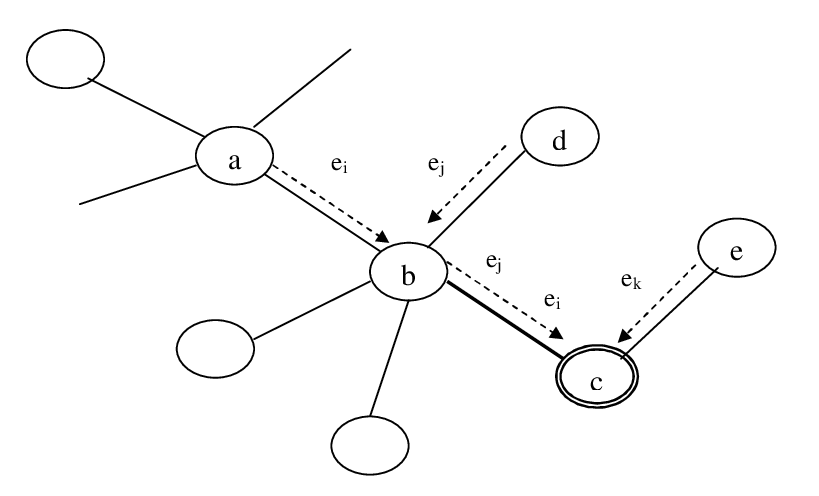
\includegraphics[width=0.8\linewidth]{yu2006_kuva}
  \caption{Havainnekuva siitä kuinka ``path reinforcement'' algoritmi pyrkii
    lähettämään toisiinsa liittyvän datan samalle nodelle.~\parencite{Yu2006}}
\label{fig:yu2006}
\end{figure}

\subsection{Vahvistusoppimisen hyödyntäminen sopeutuvassa anturiverkossa}

\begin{figure}[h]
  \centering
  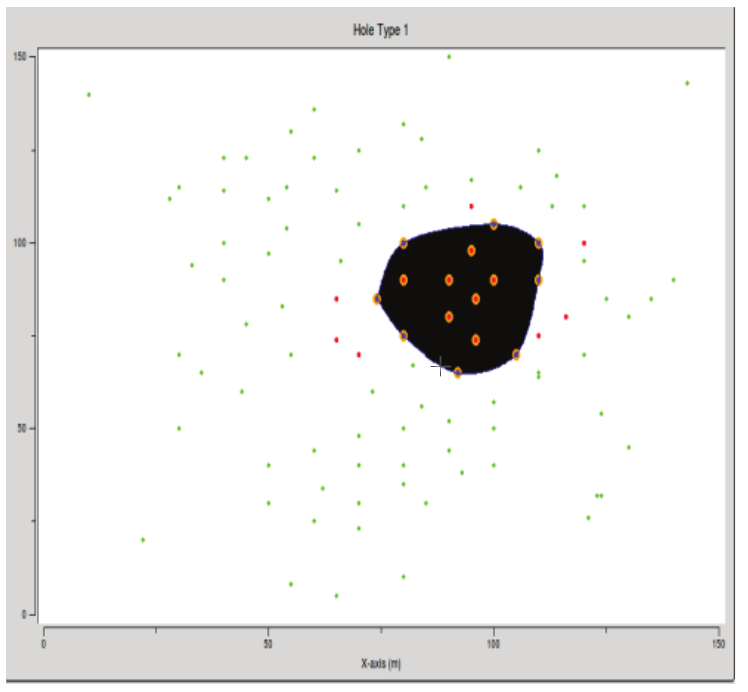
\includegraphics[width=0.8\linewidth]{arya2015_kuva}
  \caption{Simulaatiokuva artikkelissa~\cite{Arya2015} määritellystä
algoritmista. Kuvassa näkyy anturien kuolemasta syntynyt reikä mustalla.}
\label{fig:arya2015}
\end{figure}

